\documentclass[UTF8,a4paper,12pt]{ctexart}
\usepackage{ctex}
\usepackage{amsmath}
\numberwithin{equation}{section}
\allowdisplaybreaks[4]       %多行公式中换页
\usepackage{array}
\usepackage[font=small,font=bf,labelsep=none]{caption}
\usepackage{amssymb}
\usepackage{tikz}
\usepackage{amsthm}
\usepackage{mathrsfs}
\usepackage{dutchcal}
\usepackage{color}
\usepackage{graphicx}    %插入图片
\usepackage{times}
\usepackage{mathptmx}
\usepackage{fancyhdr} %页眉页脚
\pagestyle{fancy}
\fancyhf{}
\fancyfoot[C]{\thepage}
\usepackage{setspace}
\setlength{\baselineskip}{20pt}
\newcommand*{\circled}[1]{\lower.7ex\hbox{\tikz\draw (0pt, 0pt)%
    circle (.5em) node {\makebox[1em][c]{\small #1}};}}
\usepackage{hyperref}  %目录
\hypersetup{colorlinks=true,linkcolor=black}
\renewcommand {\thefigure} {\thesection{}-\arabic{figure}}%设定图片的编号。这样设置的实现效果为图1-1
\renewcommand {\thetable} {\thesection{}-\arabic{figure}}
\usepackage{caption}
\captionsetup{font={small},labelsep=quad}%文字5号,之间空一个汉字符位。
\captionsetup[table]{font={bf}} %表格表号与表题加粗
\usepackage{appendix}
\usepackage{tocloft} 
\renewcommand{\cftsecleader}{\cftdotfill{\cftdotsep}} %为目录中section补上引导点
\usepackage{titletoc}
\titlecontents{section}[0pt]{\addvspace{6pt}\filright\bf}%
               {\contentspush{\thecontentslabel \quad}}%
               {}{\titlerule*[8pt]{.}\contentspage}
\makeatletter %双线页眉
\def\headrule{{\if@fancyplain\let\headrulewidth\plainheadrulewidth\fi%
\hrule\@height 1.5pt \@width\headwidth\vskip1.5pt%上面线为1pt粗
\hrule\@height 0.5pt\@width\headwidth  %下面0.5pt粗
\vskip-2\headrulewidth\vskip-1pt}      %两条线的距离1pt
  \vspace{6mm}}     %双线与下面正文之间的垂直间距
\makeatother
\CTEXsetup[format={\heiti \zihao{3} \bfseries \center}]{section}
\CTEXsetup[number={第\chinese{section}章}]{section} 
\usepackage[explicit]{titlesec}
\titlespacing*{\section}{0pt}{24pt plus .24pt minus .24pt}{18pt plus .0ex}

\begin{document}

\thispagestyle{empty}

\renewcommand{\headrulewidth}{0pt}
\begin{figure}[htb] 
 \center{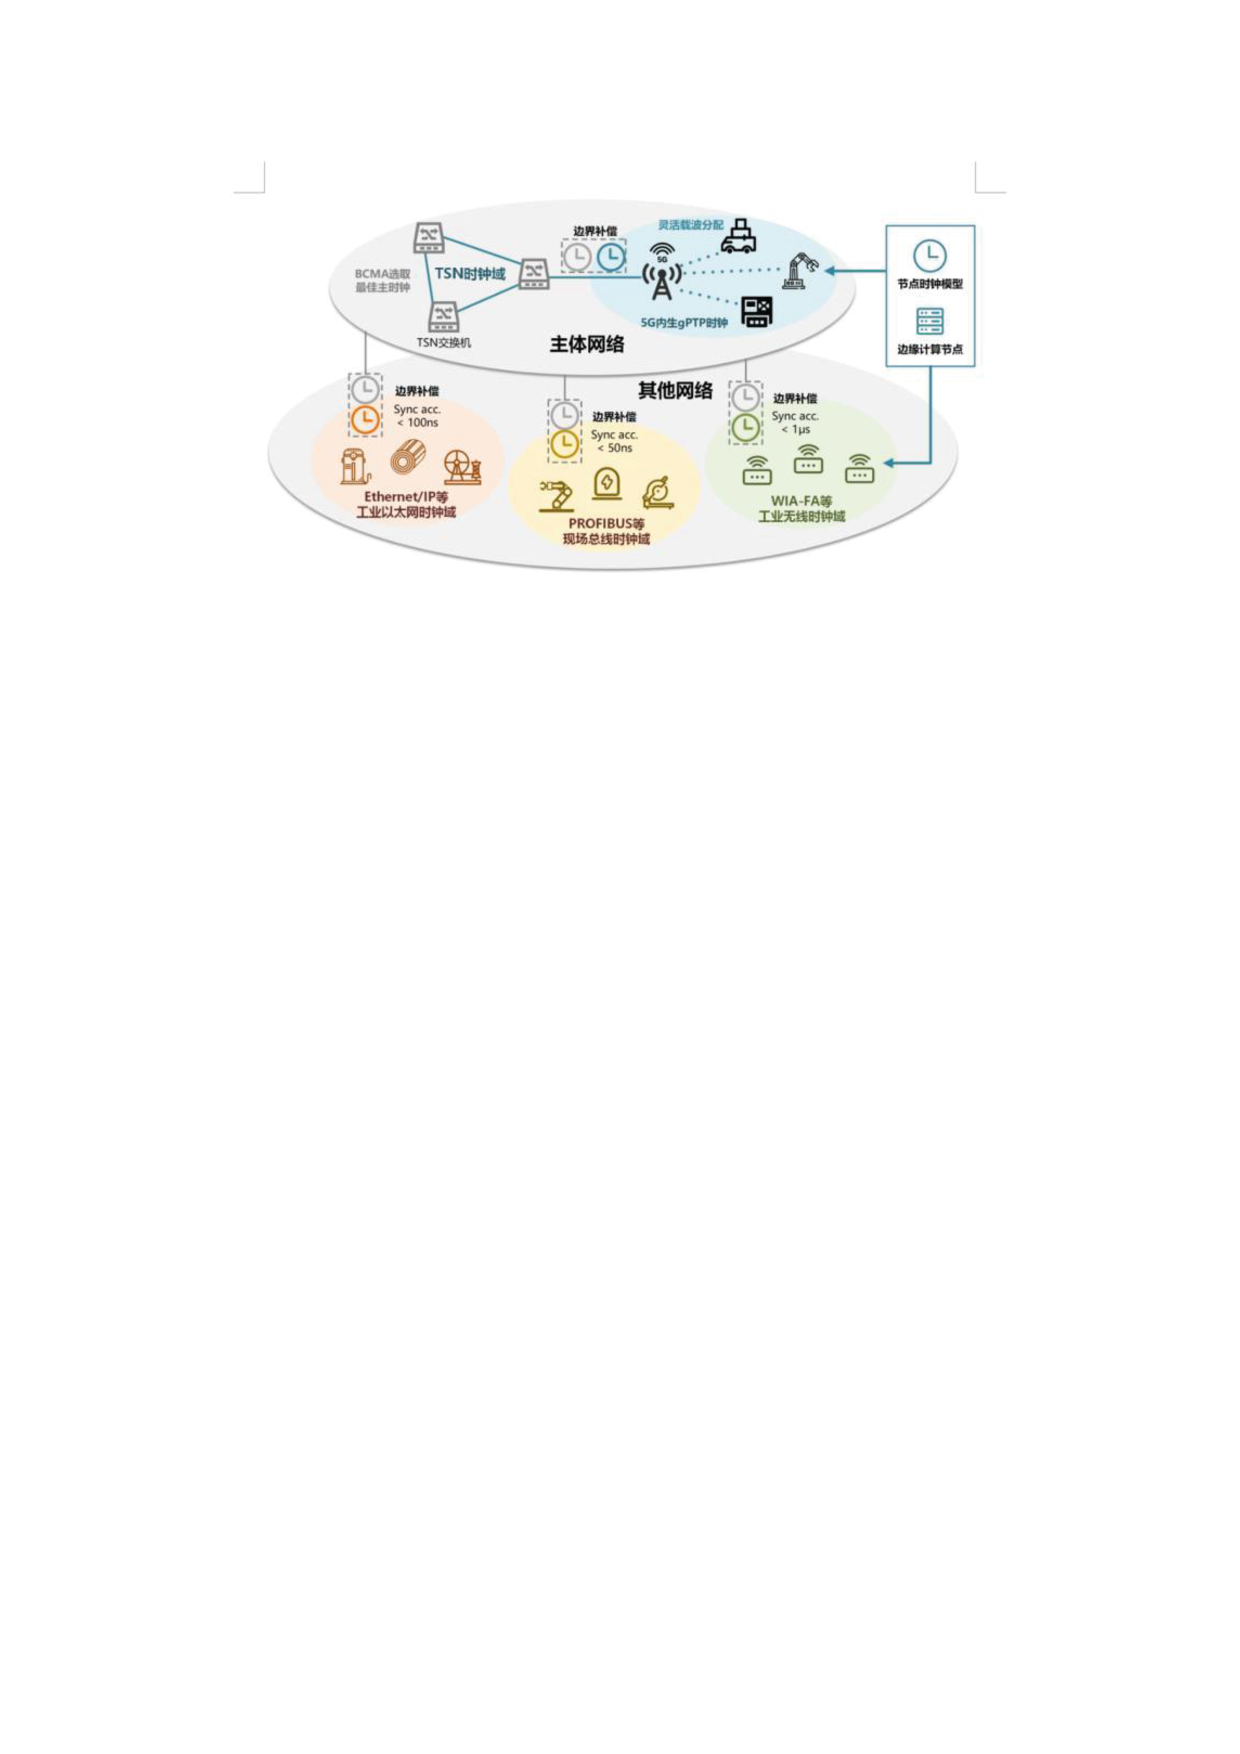
\includegraphics[width=5cm]  {fig1.png}} 
 \end{figure}

\begin{center}
\songti \zihao{-2} 上海交通大学学位论文
\end{center}
%该页为中文扉页。无需页眉页脚,纸质论文应装订在右侧
~\\
\begin{center}
\songti \zihao{1} \textbf{上海交通大学学位论文格式模板}
\end{center}
%中文论文标题,1行或2行,宋体,加粗,二号,居中。论文题目不得超过36个汉字
~\\
~\\
~\\
~\\
\begin{center}
\heiti \zihao{4}
\begin{tabular}{l}
\textbf{姓\quad名:}\\
\textbf{学\quad号:}\\
\textbf{导\quad师:}\\
\textbf{学\quad院: }\\
\textbf{学科/专业名称:}\\
\textbf{申请学位层次:}\\
\end{tabular}
\end{center}
~\\
\begin{center}
\songti \zihao{4} \textbf{20XX年XX月}
\end{center}

\newpage
\thispagestyle{empty}
~\\
\begin{center}
\zihao{4}
\textbf{
A Dissertation Submitted to \\
Shanghai Jiao Tong University for Master/Doctoral Degree}
\end{center}
~\\
\begin{center}
\zihao{-2}\textbf{
DISSERTATION TEMPLATE FOR MASTER DEGREE OF ENGINEERING IN \\
SHANGHAI JIAO TONG UNIVERSITY}
\end{center}
%英文论文标题:大写,Times New Roman,加粗,14 points,居中
~\\
~\\
~\\
\begin{center}
\zihao{3} 
Author:  \\
Supervisor:  
\end{center}
~\\
~\\
~\\
\begin{center}
\zihao{3} 
School of XXXXXXX \\
Shanghai Jiao Tong University \\
Shanghai, P.R.China \\
June 28th, 2021  
\end{center}

\newpage
\thispagestyle{empty}
\begin{center}
\heiti \zihao{3}\textbf{
上海交通大学\\
学位论文原创性声明}
\end{center}

\zihao{-4}
本人郑重声明:所呈交的学位论文,是本人在导师的指导下,独立进行研究工作所取得的成果。除文中已经注明引用的内容外,本论文不包含任何其他个人或集体已经发表或撰写过的作品成果。对本文的研究做出重要贡献的个人和集体,均已在文中以明确方式标明。本人完全知晓本声明的法律后果由本人承担。

\begin{flushright}
\begin{tabular}{l}
\zihao{4}
学位论文作者签名:\hspace{20mm}\qquad\\
\zihao{4}
日期:\qquad年\qquad月\qquad日
\end{tabular}
\end{flushright}

~\\
\begin{center}
\heiti \zihao{3}\textbf{
上海交通大学\\
学位论文使用授权书}
\end{center}

本人同意学校保留并向国家有关部门或机构送交论文的复印件和电子版,允许论文被查阅和借阅。\\
本学位论文属于 :\par
□公开论文\par
□内部论文,保密□1年/□2年/□3年,过保密期后适用本授权书。\par
□秘密论文,保密\_\_\_年(不超过10年),过保密期后适用本授权书。\par
□机密论文,保密\_\_\_年(不超过20年),过保密期后适用本授权书。\par
(请在以上方框内选择打“√”)\\

\begin{flushright}
\zihao{4}
\begin{tabular}{l l}
学位论文作者签名:\hspace{10mm}\qquad \hspace{100mm}&指导教师签名:\qquad\\
日期:\qquad年\qquad月\qquad日 &日期:\qquad年\qquad月\qquad日\\
\end{tabular}
\end{flushright}

\newpage
\pagenumbering{Roman}
\fancyhead[LH]{上海交通大学学位论文}
\fancyhead[RH]{第一章\quad绪论}

\addcontentsline{toc}{section}{摘\quad要}
\section*{摘\quad要}
%摘要:二字间空一格,黑体16磅加粗居中,单倍行距,段前24磅,段后18磅。

\hspace{8mm}学位论文是研究生从事科研工作的成果的主要表现,集中表明了作者在研究工作中获得的新的发明、理论或见解,是研究生申请硕士或博士学位的重要依据,也是科研领域中的重要文献资料和社会的宝贵财富。\par 
为了提高研究生学位论文的质量,做到学位论文在内容和格式上的规范化与统一化,特制作本模板。\\
~\\
\textbf{关键词}:学位论文,论文格式,规范化,模板\\
%关键字:宋体12磅,行距20磅,段前段后0磅,关键字之间用逗号隔开,关键词三个字加粗。

\newpage
\addcontentsline{toc}{section}{ABSTRACT}
\section*{ABSTRACT}
%ABSTRCT:Arial 16磅加粗居中,单倍行距,段前24磅,段后18磅

\hspace{8mm}As a primary means of demonstrating research findings for postgraduate students, dissertation is a systematic and standardized record of the new inventions, theories or insights obtained by the author in the research work. It can not only function as an important reference when students pursue further studies, but also contribute to scientific research and social development.\par 
This template is therefore made to improve the quality of postgraduates’ dissertation and to further standardize it both in content and in format.\\
%英文摘要内容:Times New Roman 12磅,行距20磅段前段后0磅
~\\ 
\textbf{Key words}: dissertation, dissertation format, standardization, template
%Keywords:Times New Roman 12磅,行距20磅, “key words” 两词加粗

\newpage
\renewcommand\contentsname{\textbf{目\quad录}}
\begin{center}
{\tableofcontents
\thispagestyle{fancy}
\fancyhead [RO, LE] {\normalsize{\songti 第一章\quad绪论}}
\fancyhead [LO, RE] {\normalsize{\songti 上海交通大学学位论文}}
}
\end{center}

\newpage
\pagenumbering{arabic}
\section{绪论}
\subsection{研究背景}
近年来,诸如工业自动化,IoT(Internet of Things)之类的技术增长了许多倍,应用变得至关重要。[1]云计算和高速网络的兴起要求高度精确的时间同步[2]。廉价的振荡器或石英晶体的特性会随功率,老化和热量的变化而变化。因此,不能保证两个相似的晶体以相同的时间/频率振荡。这些限制使振荡器的运行与其他振荡器略有不同。对于大型基础架构而言,用昂贵的时钟代替计算机的内置廉价时钟是不可行的。因此,一种有力而有效的方式来同步已传播结构的时钟是必不可少的[3]。NTP(Network Time Protocol)是时钟同步的最广泛使用的解决方案。后来,一种更精确的解决方案称为PTP,已被证明对时钟同步更有利[4]。尽管PTP通信算法与NTP类似,但PTP在事件的精确硬件辅助时间记录上却有所不同,称为时间戳[5]。 PTP是可以实现高精度时钟同步的一种可行解决方案。时钟同步是工业网络中非常重要的一环,而且对于时钟同步的要求也是越来越高的,其中无线和有线的时钟同步精度也是有着较大的差别。在有线领域,早期NTP的时钟同步精度由于是协议层的时间戳,误差一般达到10μs以上,再后来1588的时钟同步利用硬件时间戳,将精度提到到了几十纳秒到几十亚微秒间,同时减少了时钟同步对外部GPS信号的依赖,现在TSN(Time Sensitive Network)的802.1AS使用1588的同步方案,同时完全使用mac层的信息交互,减少了各层级之间的延迟误差,将同步精度稳定在了纳秒级,在具体的工业网络场景中,例如在现有的工业控制网络ethercat中,利用“分布时钟”机制,可以实现小于1μs的时钟同步精度。[6]在无线领域,时钟同步由于无线情况下的能量约束,本身报文时间粒度不高,传输过程中的干扰,本身同步精度要求不高等问题,精度一直停留在微秒级别。但是在5G的应用场景例如载波聚合,多点协同中,同步精度则要求达到100ns级别[7]。


TSN由于其高确定性网络而由于成为当前热门,TSN作为时间敏感网络,拥有诸如Qbv等门控调度算法保护来保证时间敏感流的传输,现在做调度算法的有很多,但有一个假设前提:时钟同步是完美的,不存在同步误差和误差抖动;但是,在实际工业场景中假设不成立。TSN对于时钟同步的精度要求极高(ns级别),目前的TSN的同步协议802.1AS,在可接受的误差范围内,有线网络可以提供高精度的时钟同步,但是当网络规模较大,跳数增多,背景流量增多时,同步精度会大幅下降,从而影响整个TSN的性能。[8]换言之,TSN本身收到有线网络的局限性,需要通过与无线异构来解决有线跳数过多的问题,且在工厂内部的复杂环境下,本身就可能存在的多种无线设备与有线设备异构的情况,仅仅通过保证TSN有线网络内部的高精度同步无法满足实际的应用场景。为将TSN和无线网络相互结合,需要进一步考虑异构网络下的时钟同步方法,可以通过双层网络架构来降低网络规模对于整个同步精度的影响,也就是TSN+无线解决方案,即上层GM(Grand Master)到基站采用有线TSN结构,下层采用无线网络来同步从节点,这种情况下,无线网络的高覆盖性,可以有效降低网络规模较大的情况下跳数对于同步精度的影响,为TSN提供了一个更加有实际意义的应用场景。


针对这种有线无线网络异构结构,这些年也有很多时钟同步方案被提出,用来解决异构网络的协同问题,不同的同步方法有着其适用的范围,而对于大规模无线网络节点的异构同步方案,目前没有比较好的同步解决方案。

\subsection{研究现状}
为解决异构网络的同步问题,通常都会选择选择先优化有线网络同步精度,将其作为主时钟后再针对无线网络进行主从同步。
有线网络部分的时钟同步,目前精度最高的有线网络同步为时间敏感网络的同步方案,时间敏感网络(Time Sensitive Network),简称TSN,采用TSN中协议802.1AS规定的时钟同步方案,此此方案是根据1588时钟同步方案改进而来,采用主从式同步方法,主从节点之间通过交换时间戳进行上下行延迟进行测量,得到两节点之间的传输延迟,进一步得到时钟偏差。事实上,两节点之间的传输延迟由报文传播延迟,高斯噪声,不确定性延迟组成,后两者是造成时钟同步精度误差的主要原因。在有线网络中,由于较高的稳定性和较好的传输性能,这两部分一般选择忽略不计,即将上下行传输延迟作为对称延迟来进行处理。[8]


相比于有线情况的时钟同步,无线网络中的能量约束,以及节点之间的传输干扰,造成无线时钟同步的误差较大。高精度的无线时钟同步的研究目前主要针对WSN和5G。

如果是倾向于高精度的无线时钟同步方案,在同步方法上,更多是采用类似1588的上下报文测量传输延迟的同步方案,在网络结构上,更多是采用类似于聚类的网络结构。聚类网络结构时钟同步的出发角度有从能量的角度出发进行考虑的,也有单纯从精度的角度出发进行考虑的。精度的方面,Xiangli Jia和Yang Lu针对网络跳数对于同步精度的影响做了专门的分析,得出了聚类网络结构相对于传统多跳网络结构的优势[9]。Jie Wu,Liyi Zhang则在聚类网络的结构基础上,提出了通过计算共识时钟来进行同步的方案。从能量的角度出发进行考虑的聚类网络结构,更多是从聚类算法的角度进行研究[10]。Pengyi Jia提出通过时钟频率抖动的大小s来进行网络聚类,通过将性能较差的时钟节点聚类进行同步的方式,可以有效降低网络整体的时钟同步频,从而达到降低网络整体能耗的目的[11]。Parminder Kaur也在文章中提出可以通过就近原则的聚类方法,来降低所有节点间通信距离差的和,来达到降低能耗的目的[12]。


针对传统的WSN网络中的聚类时钟同步在现实的应用问题,文献 [13] 等人研究了这些聚类结构时钟同步在5G中的可行性,并提出了可能存在的挑战以及可能的解决方案。5G下的时钟同步,主要是通过BS来完成上层与下层网络之间的同步。但是目前用来传输时间信息的报文SIB16时间精度不高,这就造成了影响时间同步精度关键的时间戳精度不高,而且无线时钟同步方案的时间戳采用的是应用层的时间戳,应用层时间戳在产生过程中很可能会产生较大的非确定性延迟,例如排队延迟,这类延迟通常数量级较大,在传统时钟同步方案中由于产生概率较低,通常放弃对这部分延迟的建模,但是当网络规模增大时,这类延迟的产生概率也会随着增加,从而对时钟同步精度产生较大的影响。如果要实现像TSN的802.1AS一样的高精度时间同步,必须对这一类延迟进行建模补偿,从而才能使得无线网络和有线TSN时钟同步实现对接。 


在很多研究中,无线网络只是作为一个性能较差的有线网络来进行建模,所谓的异构网络,仅仅只是两个性能不同的有线网络连接在一起,然而事实上,根据文献[14],[15]所述,无线网络和有线网络对接的过程中,之所以会产生较大的同步误差,很大原因是由于在上行回传的过程中,会产生较大的PDV(packet delay variation),从而严重影响同步性能。众所周知,定时数据包中的PDV(即延迟抖动)是降低IEEE 1588系统中同步精度的主要因素。 PDV是由于交换集线器上的数据包排队而产生的。 例如,在具有快速以太网接口的交换集线器中,如果在时序数据包到达时仅一个最大传输单元(MTU)大小为1518字节的数据包位于缓冲区中,则排队延迟最多变化122.4μs。这显然会较大地影响同步性能,造成有线网络和无线网络部分的对接困难。即不能很好地实现5G和有线TSN的对接。
为了克服由于延迟抖动引起的同步性能的下降,已经广泛研究了各种同步过程。文献[16],[17]具有以太滤波方法或统计方法的反馈回路是一种基本机制。但是,反馈系数是根据经验确定的。因此,通常很难自适应地优化它们。因此,就稳定性和准确性而言,可能难以获得足够的同步性能。


文献[18],[19]为了减轻由于延迟抖动引起的同步精度下降,提出了一种使用探测数据包进行排队估计的方法。采用探测数据包的目的是估计定时数据包中延迟抖动的发生,并且 过滤出具有时延抖动的数据包。这种方法可以有效测出当前的实际网络排队延迟大小,但是过程过于繁琐,且容易造成新增流量过多,能耗增大的问题。


文献[20],[21]指出诸如IEEE 1588精确时间协议和网络时间协议之类的时序协议要求对时间服务器(主服务器)与客户端(从属服务器)之间的通信路径延迟进行精确测量,以提供精确的时序同步。然后,使用这样的假设来估计客户站点上的准确时间,该假设是由于通过网络的物理传播时间引起的前向和后向延迟相等,或者它们之间的任何差异都是预先校准的。除了物理链路延迟之外,由于路径上的交换/路由设备,定时数据包还会遇到队列引起的延迟。将排队延迟归于非对称延迟中,并针对齐设计了补偿算法。但是其补偿算法依然依赖每次测量得到的数据,对于时钟同步来说过于繁琐。


文献[22]指出基于经典双向消息交换方案的IEEE 1588是用于分组交换网络的流行时钟同步协议。由于数据包交换网络中存在随机排队延迟,因此时钟偏斜和与已交换同步数据包时间戳之间的偏移的联合恢复可以视为统计估计问题。在前向主从路径与反向从主路径的确定性路径延迟之间可能存在未知性的情况下,IEEE 1588的时钟偏斜和偏移估计问题来自不正确的建模或网络攻击。首先,假设多个主从通信路径的可用性以及对描述随机排队延迟的概率密度函数的全面了解,该文章针对IEEE 1588的时钟偏斜和偏移估计方案,针对均方估计误差开发了下限。通过混合高斯随机变量来近似随机排队延迟的概率密度函数,该文章提出了一种鲁棒的迭代时钟偏斜和偏移估计方案,该方案采用空间交替广义期望最大化(SAGE)算法来学习所有未知参数。数值结果表明,所开发的鲁棒方案显示出接近下限的均方估计误差。这篇文章通过引入高斯混合分布来对排队延迟建模来达到了更好的时钟偏差估计,但整个计算过程过于复杂,传输开销较大。


实际应用过程中,由于5G网络低延迟,高精度的特性,是最有可能成为未来无线TSN载体的通信协议。目前针对5G和TSN融合的问题,3GPP协议和各通信厂商给出的解决方案为5G网桥。通过CNC对5G网络分配网桥的角色,并在有线无线交接处的协议转换器记录时间戳来计算5G网络内部的驻留时间,从而实现5G网络两端的TSN有线设备满足同步要求。但是该方案并不能满足未来无线TSN设备的同步需求,因为其并没有解决无线网络内部的累积同步误差问题,会使得同步精度偏低。


综上所述,目前5G网络对于时钟同步虽然提出了具体的要求,但是还缺乏具体的解决方案,尤其是对于未来高精度的无线时钟同步应用场景,例如以5G为媒介的大规模的无线TSN网络,现有的解决方案往往存在精度较低或者计算过于复杂,同步效率较低的情况。
\subsection{引言}
学位论文……
\subsection{本文主要研究内容}
本文……
\subsection{本文研究意义}
本文……
\subsection{本章小结}
本文……

\newpage
\fancyhead[LH]{上海交通大学学位论文}
\fancyhead[RH]{第二章\quad正文文字格式}
\section{正文文字格式}
\subsection{论文正文}
论文正文是主体,一般由标题、文字叙述、图、表格和公式等部分构成。一般可包括理论分析、计算方法、实验装置和测试方法,经过整理加工的实验结果分析和讨论,与理论计算结果的比较以及本研究方法与已有研究方法的比较等,因学科性质不同可有所变化。\par
论文内容一般应由十个主要部分组成,依次为:⒈封面,⒉中文摘要,⒊英文摘要,⒋目录,⒌符号说明,⒍论文正文,⒎参考文献,⒏附录,⒐致谢,⒑攻读学位期间发表的学术论文目录。\par
以上各部分独立为一部分,每部分应从新的一页开始,且纸质论文应装订在论文的右侧。\par
\subsection{字数要求}
\subsubsection{硕士论文字数要求}
各学科和学部自定
\subsubsection{博士论文字数要求}
各学科和学部自定
\subsection{本章小结}
本章介绍了……

\newpage
\fancyhead[LH]{上海交通大学学位论文}
\fancyhead[RH]{第三章\quad图表、公式格式}
\section{图表、公式格式}
\subsection{图表格式}

\begin{figure}[htb] 
\center{\includegraphics[width=0.95\textwidth]  {fig2.png}} 
\caption{内热源沿径向的分布}
\end{figure}

\begin{table}[!htbp]
\centering
\caption{高频感应加热的基本参数}
\begin{tabular}{|c| c|c|c|}
\hline
感应频率 &感应发生器功率 & 工件移动速度  &感应圈与零件间隙\\
(KHz)&($\% \times$80Kw) &(mm/min)  &(mm)\\
\hline
250 &88 &5900 &1.65\\
\hline
250 &88 &5900 &1.65\\
\hline
250 &88 &5900 &1.65\\
\hline
250 &88 &5900 &1.65\\
\hline
250 &88 &5900 &1.65\\
\hline
250 &88 &5900 &1.65\\
\hline
250 &88 &5900 &1.65\\
\hline
250 &88 &5900 &1.65\\
\hline
\end{tabular}
\end{table}

\begin{table}
\centering
\captionsetup{singlelinecheck=off}
\caption*{续表} %取消编号
\begin{tabular}{|c| c|c|c|}
\hline
感应频率 &感应发生器功率 & 工件移动速度  &感应圈与零件间隙\\
(KHz)&($\% \times$80Kw) &(mm/min)  &(mm)\\
\hline
250 &88 &5900 &1.65\\
\hline
250 &88 &5900 &1.65\\
\hline
\end{tabular}
\end{table}
%表格太大需要转页时,需要在续表上方注明“续表”,表头也应重复排出。


\subsection{公式格式}

\vspace{-10mm}
\begin{eqnarray}
\frac{1}{\mu} \nabla^2A - j \omega \sigma A -\nabla(\frac{1}{\mu}) \times(\nabla \times A)+J_0=0
\end{eqnarray}

\subsection{本章小结}
本章介绍了……

\newpage
\fancyhead[LH]{上海交通大学学位论文}
\fancyhead[RH]{第四章\quad全文总结}
\section{全文总结}

\subsection{主要结论}
本文主要……

\subsection{研究展望}
更深入的研究……

\newpage
\fancyhead[LH]{上海交通大学学位论文}
\fancyhead[RH]{参考文献}

\addcontentsline{toc}{section}{参\quad考\quad文\quad献}
\renewcommand\refname{参\quad考\quad文\quad献}
\begin{thebibliography}{1}
\bibitem{1} 杨瑞林, 李力军. 新型低合金高强韧性耐磨钢的研究. 钢铁. 1999(7):41~45.
\bibitem{2}  Schinstock, D.E., Cuttino, J.F. Real time kinematic solutions of a non-contacting, three dimensional metrology frame[J]. Precision Engineering. 2000, 24(1):70-76. 
\bibitem{3} 温诗铸. 摩擦学原理. 北京:清华大学出版社. 1990:296-300.
\bibitem{4} 贾名字. 工程硕士论文撰写规范[硕士论文].上海:上海交通大学. 2000.
\bibitem{5} 姜锡洲.一种温热外敷药制备方案[P].中国专利:881056078,1983-08-12.
\bibitem{6}]GB/T16159—1996,汉语拼音正词法基本规则[S].北京:中国标准出版社,1996.
\end{thebibliography}

\newpage
\fancyhead[LH]{上海交通大学学位论文}
\fancyhead[RH]{附录1}

\addcontentsline{toc}{section}{附录}
\section*{符号与标记(附录1)}

\newpage
\fancyhead[LH]{上海交通大学学位论文}
\fancyhead[RH]{学术论文和科研成果目录}

\addcontentsline{toc}{section}{攻读学位期间学术论文和科研成果目录}
\section*{攻读学位期间学术论文和科研成果目录}

[1] 张三,李四. …… (已录用)

\newpage
\fancyhead[LH]{上海交通大学学位论文}
\fancyhead[RH]{致\qquad谢}

\addcontentsline{toc}{section}{致\qquad谢}
\section*{致\qquad谢}

\hspace{8mm}致谢主要感谢导师和对论文工作有直接贡献和帮助的人士和单位。致谢言语应谦虚诚恳,实事求是。





\end{document} 